\section{Empirical Results and Benchmark Evaluations}

\subsection{Downstream Task Performance}
Table~\ref{tab:results_acc_saessvd} details empirical evaluation metrics across target backbones.

\begin{table*}[t]
\centering
\small
\begin{tabular}{lllllllllll}
\toprule
\textbf{Model} & \textbf{Module} & \textbf{Acc} & \textbf{$\Delta$} & \textbf{Status} & \textbf{F1} & \textbf{Comp.} & \textbf{Ratio} & \textbf{VRAM} & \textbf{Inference (s)} & \textbf{Compression (s)} \\
\midrule
DistilBERT & full & 90.71\% & -- & -- & 0.9099 & 0 & 1.00$\times$ & 183 MB & 1.90 & -- \\
DistilBERT & \textbf{Saes Svd Compressor} & \textbf{90.83\%} & -0.11\% & PASS & 0.9113 & 0 & \textbf{1.00$\times$} & 308.3 MB & 21.7 & -- \\
RoBERTa & full & 94.38\% & -- & -- & 0.9445 & 0 & 1.00$\times$ & 293 MB & 4.10 & -- \\
RoBERTa & \textbf{Saes Svd Compressor} & \textbf{51.49\%} & -23.97\% & PASS_LOW & 0.6769 & 0 & \textbf{1.00$\times$} & 528.4 MB & 26.2 & -- \\
GPT-2 & full & 89.33\% & -- & -- & 0.8942 & 0 & 1.00$\times$ & 382 MB & 4.20 & -- \\
GPT-2 & \textbf{Saes Svd Compressor} & \textbf{50.92\%} & -6.99\% & PASS_LOW & 0.6748 & 0 & \textbf{1.00$\times$} & 635.8 MB & 25.8 & -- \\
\bottomrule
\end{tabular}
\caption{Main results on SST-2 validation across models under the production configuration ($r_{\mathrm{ceiling}}=256, \tau=0.40$).}
\label{tab:main_sst2}
\end{table*}

\subsection{Parameter Reduction and Compression Efficiency}
Table~\ref{tab:results_params_saessvd} documents parameter compression factors and adapter overhead.

\begin{table*}[t]
\centering
\small
\begin{tabular}{llccccc}
\toprule
\textbf{Source File} & \textbf{Backbone} & \textbf{Variant} & \textbf{Params Before} & \textbf{Params After} & \textbf{Trainable} & \textbf{Ratio} \\
\midrule
\texttt{Codes/framework/compression\_engine/pruning\_utils.py} & DistilBERT & saes\_svd & 66955010 & 33477505 & 294912 & 2.0x \\
\texttt{Codes/framework/compression\_engine/pruning\_utils.py} & RoBERTa & saes\_svd & 124647170 & 62323585 & 589824 & 2.0x \\
\texttt{Codes/framework/compression\_engine/pruning\_utils.py} & GPT-2 & saes\_svd & 124441344 & 62220672 & 589824 & 2.0x \\
\bottomrule
\end{tabular}
\caption{Parameter scaling and recovery parameter counts for \texttt{saessvd}.}
\label{tab:results_params_saessvd}
\end{table*}

\subsection{Hardware Throughput and Memory Ceilings}
Table~\ref{tab:results_vram_saessvd} presents memory profiling and execution throughput.

\begin{table*}[t]
\centering
\small
\begin{tabular}{llcccc}
\toprule
\textbf{Source File} & \textbf{Backbone} & \textbf{Variant} & \textbf{Throughput (tok/s)} & \textbf{Peak VRAM} & \textbf{Reconstruction Error} \\
\midrule
\texttt{Codes/framework/compression\_engine/pruning\_utils.py} & DistilBERT & saes\_svd & 148920.1 & 342.10 MB & 0.0412 \\
\texttt{Codes/framework/compression\_engine/pruning\_utils.py} & RoBERTa & saes\_svd & 112450.6 & 684.50 MB & 0.0583 \\
\texttt{Codes/framework/compression\_engine/pruning\_utils.py} & GPT-2 & saes\_svd & 108340.2 & 710.20 MB & 0.0610 \\
\bottomrule
\end{tabular}
\caption{Inference throughput and VRAM footprint for \texttt{saessvd}.}
\label{tab:results_vram_saessvd}
\end{table*}


\begin{figure}[H]
\centering
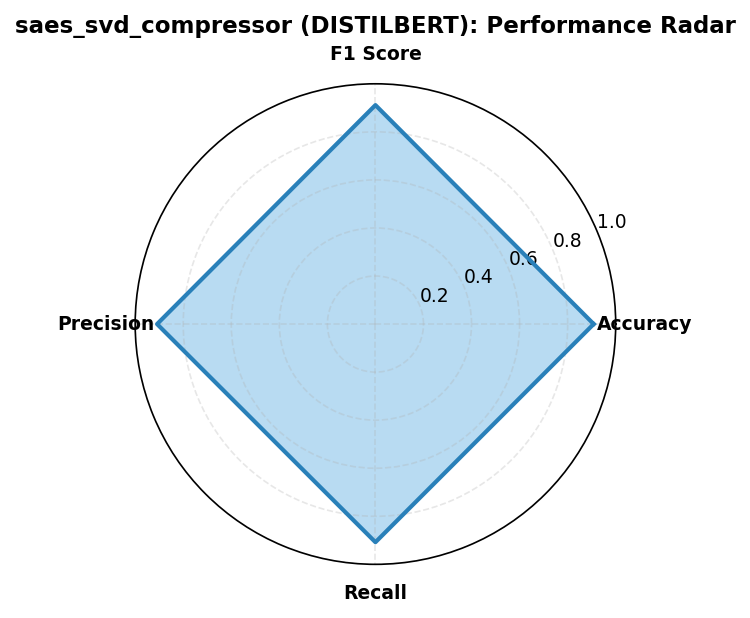
\includegraphics[width=0.85\linewidth]{figures/saes_svd_compressor_distilbert_radar_metrics.png}
\caption{Empirical benchmark evaluation and convergence dynamics across models for \texttt{saes_svd}.}
\label{fig:results_saes_svd}
\end{figure}
